\section{Composite}

The composite pattern describes a group of objects that is treated the same way as a single instance of the same type of object. The intent of a composite is to ``compose" objects into tree structures to represent hierarchies. Implementing the composite pattern lets clients treat individual objects and compositions uniformly.

\subsection*{Example}

Figure~\ref{fig:composite} presents the composite design pattern found in the project \textit{lotus}. The interface \texttt{Decision} plays the role of \textit{Component}, the class \texttt{MultiDecision} plays the role of \textit{Composite}, and the classes \texttt{PassDecision} and \texttt{PlayLand} plays the role of \textit{leaf}.

\begin{figure}[htb]
    \centering
    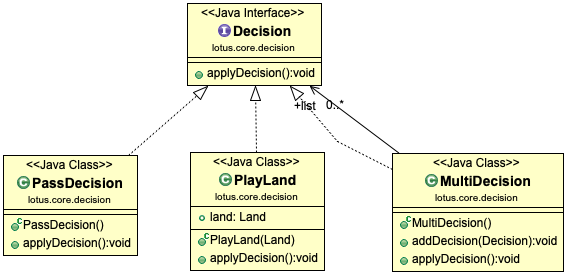
\includegraphics[width=0.8\columnwidth]{images/composite.png}
    \caption{Composite design pattern in the project \textit{lotus}}
    \label{fig:composite}
\end{figure}
\FloatBarrier

%--------------------------------------------------------------------------------------------%

An instance of the client manages the decision of the player. A decision is an action decided by the player. Figure~\ref{fig:Decision} presents the implementation of the interface \texttt{Decision} that contains only one method that applies the decision of the player.

\begin{figure}[!tbp]
\centering
\lstset{language=Java,  basicstyle=\scriptsize, stepnumber=1, showspaces=false, showstringspaces=false,breaklines=true}
\begin{lstlisting}

public interface Decision{
	public void applyDecision();
}

\end{lstlisting}
\caption{[Composite] Decision.java}
\label{fig:Decision}
\end{figure}
\FloatBarrier

%--------------------------------------------------------------------------------------------%
Figure~\ref{fig:MultiDecision} presents the implementation of the class \texttt{MultiDecision} that implements the interface \texttt{Decision}. This class represents multiple decisions as one decision.

\begin{figure}[!tbp]
\centering
\lstset{language=Java,  basicstyle=\scriptsize, stepnumber=1, showspaces=false, showstringspaces=false,breaklines=true}
\begin{lstlisting}
public class MultiDecision implements Decision {
	public ArrayList<Decision> list = new ArrayList<Decision>();
	
	public void addDecision(Decision d) {
		list.add(d);
	}
 
	public void applyDecision() {
		for(Decision d : list) {
			d.applyDecision();
		}
	}
}
\end{lstlisting}
\caption{[Composite] MultiDecision.java}
\label{fig:MultiDecision}
\end{figure}
\FloatBarrier

%--------------------------------------------------------------------------------------------%
Figure~\ref{fig: PlayLand} presents the implementation of the class \texttt{PlayLand} that also implements \texttt{Decision}. In this class, the player decided to play a land.

\begin{figure}[!tbp]
\centering
\lstset{language=Java,  basicstyle=\scriptsize, stepnumber=1, showspaces=false, showstringspaces=false,breaklines=true}
\begin{lstlisting}

public class PlayLand implements Decision {
	public Land land;
	public PlayLand(Land l) {
		land = l;
	}
	public void applyDecision() {
		ChangeZone eff = new ChangeZone(land,land.zone,land.owner.inPlay);
		eff.resolve();
	}
}
\end{lstlisting}
\caption{[Composite] PlayLand.java}
\label{fig: PlayLand}
\end{figure}
\FloatBarrier

%--------------------------------------------------------------------------------------------%
Figure~\ref{fig:PassDecision} presents the implementation of the class \texttt{PassDecision} that also implements \texttt{Decision}. In this class, the played decided do anything, i.e., pass the decision.

\begin{figure}[!tbp]
\centering
\lstset{language=Java,  basicstyle=\scriptsize, stepnumber=1, showspaces=false, showstringspaces=false,breaklines=true}
\begin{lstlisting}

public class PassDecision implements Decision {
	public void applyDecision() {
		// Decision to pass, ie do nothing
	}
}

\end{lstlisting}
\caption{[Composite] PassDecision.java}
\label{fig:PassDecision}
\end{figure}
\FloatBarrier

%--------------------------------------------------------------------------------------------%